\documentclass[dissertation.tex]{subfiles}
\begin{document}

\chapter{Comparative genomics}
\label{chap:comparative}

Outline ideas:
\begin{itemize}
  \item Introduction / overview:
  \begin{itemize}
    \item The use of models in PC (very brief)
    \item Specific models used in PC, with strong focus on the most common (KPC), and derivates.  Cover ease-of-use briefly.
    \item Current knowledge re: how appropriate the models are.  Consider histology, genetic features, disease progress (incl. metastatic potential), response to therapy.  Highlight gap in genetic information, and relevance to response to therapy.
    \item Brief overview of known genetic features of human disease.  Raise possibility of subtypes.
    \item Wrap-up with overview of project:
    \begin{enumerate}
      \item Collect matched tumour-normal DNA from a range of GEMMs.
      \item Sequence and determine conserved model-specific and general patterns of somatic mutation.
      \item Compare observed patterns to human disease.
      \begin{itemize}
        \item Are genetic features of human disease recapitulated generally in the models?
        \item Does a single model match the genetic features of human disease much better than the others?
        \item Do specific models serve as simulations of certain subtypes of human disease?
      \end{itemize}
    \end{enumerate}
    \item Overall thesis for this work: \\
    Matching patterns of genetic alterations in mouse models of pancreatic cancer to those seen in human disease can inform researchers as to which models are generally best, and which best match specific patient types. \\
    Sub-theses:
    \begin{itemize}
      \item The patterns of mutations seen in common mouse models of pancreatic cancer match those consistently seen in human disease.
      \item Different mouse models possess different mutation spectra, and models may be close fits to specific genetic subtypes of patients.
    \end{itemize}
  \end{itemize}
  
  \item Results
  \begin{enumerate}
    \item Somatic SNV and indels
    \item CNV and LOH
  \end{enumerate}

  \item Conclusion
  
\end{itemize}

\section{Methods}

\subsection{Models}

\subsection{Sample Origin and Processing}

\subsection{Sequencing}

\subsection{QC}

\subsection{Mapping}

For initial mapping, all lanes were processed independently.  SHRiMP was used to map colourspace reads to the mm10 genome using `all-contigs' and `single-best-mapping' options.  Unpaired reads in the source fastq files were mapped as single reads; paired reads were mapped with pair mode `opp-in', and a per-fastq insert size distribution estimated from a normal distribution fit to insert sizes of the first 10,000 reads.  Likely duplicate reads were marked using Picard MarkDuplicates on each individual lane \gls{BAM}, using an optical duplicate pixel distance parameter of 10.

Lane \glspl{BAM} were progressively merged: first, duplicate lane \glspl{BAM} for a given mouse and sample type (tumour or normal) were combined, then tumour and normal \glspl{BAM} for a given mouse, and finally combined tumour-normal \glspl{BAM} for all mice.  Prior to each level of merging, the \gls{GATK} was used to separately perform \gls{LABQSR} on each input \gls{BAM}.  Finally, the full experiment \gls{BAM} file was recalibrated with \gls{LABQSR}, and then split by mouse and sample type for analysis, yielding 62 paired tumour and normal final \glspl{BAM}.

\subsection{Somatic SNV and Indel Detection}

muTect and Strelka were used separately to detect somatic \glspl{SNV} and \glspl{indel} in individual mouse tumour and normal \glspl{BAM}.  muTect was supplied default parameters; Strelka used the parameter settings given in listing \ref{lst:comp_strelka_settings}; these are the default parameters as recommended for use with the BWA mapper, with the exception that in this work isSkipDepthFilters was set to 1.

\begin{lstlisting}[caption=Strelka configuration file used for SNV / indel detection,label=lst:comp_strelka_settings]
[user]
isSkipDepthFilters = 1
maxInputDepth = 10000
depthFilterMultiple = 3.0
snvMaxFilteredBasecallFrac = 0.4
snvMaxSpanningDeletionFrac = 0.75
indelMaxRefRepeat = 8
indelMaxWindowFilteredBasecallFrac = 0.3
indelMaxIntHpolLength = 14
ssnvPrior = 0.000001
sindelPrior = 0.000001
ssnvNoise = 0.0000005
sindelNoise = 0.000001
ssnvNoiseStrandBiasFrac = 0.5
minTier1Mapq = 20
minTier2Mapq = 5
ssnvQuality_LowerBound = 15
sindelQuality_LowerBound = 30
isWriteRealignedBam = 0
binSize = 25000000
\end{lstlisting}


\subsection{CNV and LOH Detection}

Overview:
\begin{itemize}
  \item Very brief background of CNV and LOH in tumours, and the possibility of detection from NGS data.  Maybe pull in the hallmarks paper, or perhaps specific PC / GEMM examples.
  \item Brief overview of existing techniques and why unsuited?
  \begin{itemize}
    \item CNV:
    \begin{itemize}
      \item Exome pulldown complication
      \item Ill-posed nature of problem
      \item Human-specific methods
      \item Outbred population-specific methods
    \end{itemize}
    \item LOH:
    \begin{itemize}
      \item That Bayesian thing.  Unfortunately affected by CNV, which is unknown.
    \end{itemize}
  \end{itemize}
\end{itemize}


\subsubsection{Loss of heterozygosity at individual loci}

This work took a simple approach to identify loci with significant evidence of \gls{LOH} in a tumour sample: locate high-confidence heterozygous loci in matched normal DNA, and then test only these heterozygous loci for a significant change in allelic fraction between matched tumour and normal samples.  In regions of the genome with ploidy $2n$ and below, such allelic imbalance is indicative of \gls{LOH}, even in the presence of unknown levels of diploid genome contamination.

\paragraph{Identifying heterozygous loci in normal DNA}

High-confidence heterozygous loci in normal DNA were identified by comparing posterior genotype likelihoods using a \gls{BMC} approach.  \gls{BMC} is a procedure for deciding which of two competing models is better favoured by the observed data; here the two models are, for a given locus: `the locus is homozygous' (model $HOM$), and `the locus is heterozygous' (model $HET$).  The likelihoods of these two models (assessed on the reads observed at a locus) can be used to calculate a Bayes factor, which encodes which of the two models is better supported by the data at that locus, and how strongly.  More formally, we partition the ten possible diploid genotypes at a locus into two classes, $Hom$ and $Het$:
\begin{align}
Hom &= \{AA, CC, GG, TT\} \\
Het &= \{AC, AG, AT, CG, CT, GT\}
\end{align}
The two models, $HOM$ and $HET$, may be written
\begin{align}
HOM &: G \in Hom \\
HET &: G \in Het
\end{align}
where $G$ is the true genotype at the locus.  The Bayes factor $K$ comparing $HOM$ and $HET$ is then
\begin{align}
K &= \frac{\mathcal{L}(HET)}{\mathcal{L}(HOM)} \\
  &= \frac{Pr(D|G \in Het)}{Pr(D|G \in Hom)} \\
  &= \frac{\sum_{g \in Het} Pr(D|G = g)Pr(G = g|G \in Het) }{\sum_{g \in Hom} Pr(D|G = g)Pr(G = g|G \in Hom) }
\label{eq:comm_het_bayes}
\end{align}
with $D$ being the reads at the locus.  We make the simplifying assumption that all genotypes in each of $Hom$ and $Het$ are equally likely, so that all $Pr(G = g|G \in X) = \frac{1}{\|X\|}$ for $X \in \{Hom, Het\}$.  Then
\begin{align}
K &= \frac{\frac{1}{\|Het\|}\sum_{g \in Het} Pr(D|G = g)}{\frac{1}{\|Hom\|}\sum_{g \in Hom} Pr(D|G = g)} \\
  &= \frac{\frac{1}{\|Het\|}\sum_{g \in Het} \mathcal{L}(G = g|D)}{\frac{1}{\|Hom\|}\sum_{g \in Hom} \mathcal{L}(G = g|D)}
\end{align} 
encodes the weight of evidence for the observed read data $D$ favouring a locus being heterozygous over homozygous, and a value exceeding a given threshold is taken as significant evidence that the locus under consideration is heterozygous.

An implementation of the above heterozygous locus detection method is given in algorithm \ref{alg:comp_find_het}.  The input posterior genotype likelihoods $\mathcal{L}(G = g|D)$ are supplied by \lstinline|samtools mpileup -q 20 -Q 20 -v -u| operating on per-mouse normal sample \glspl{BAM}, and the minimum value of $K$ for a locus to be called as heterozygous is $\exp(minscore)$.  Two additional filters are also employed in the algorithm: a locus is \emph{not} reported as heterozygous if either the total read depth at the locus is less than $mindepth$, or if the difference in samtools-supplied log likelihood between the top two genotypes is less than $mindelta$ nats.  The latter filter is used to exclude any problem loci with an apparent triallelic state.  \mpfatal{give instantiation values for the algo somewhere}

\begin{algorithm}
  \KwData{Total sequence depth at the locus $D$, minimum depth for call $mindepth$, list of alternate alleles $A$, list of Phred-scaled genotype likelihoods $L$, minimum likelihood difference in nats between top two genotypes $mindelta$, minimum Bayes factor in nats for heterozygous to be called over homozygous $minscore$.}
  \KwResult{A boolean: true if the locus is called heterozygous, false if it is not.}

  \Begin {
    \If {$D \leq mindepth$}{
      \KwRet false\;
    }
    \tcp{Convert Phred-scaled likelihoods to nats}
    \For{$i \leftarrow 1$ \KwTo $\|L\|$}{
      $L_i \longleftarrow -\frac{1}{10} \log(10) L_i$\;
    }
    \tcp{Ensure the likelihood difference between the two most likely genotypes is at least $mindelta$.}
    $L^* \longleftarrow L$ sorted in decreasing order\;
    \If {$L^*_1 - L^*_2 \le mindelta$}{
      \KwRet false\;
    }
    \tcp{Calculate combined likelihoods for heterozygous and homozygous genotypes}
    \Switch{$\|A\|$}{
      \Case{$2$}{
        $L_{het} \longleftarrow L_2$\;
        $L_{hom} \longleftarrow \log\left(\frac{1}{2}\sum_{i \in \{1, 3\}} \exp(L_i) \right)$\;
      }
      \Case{$3$}{
        $L_{het} \longleftarrow \log\left(\frac{1}{6}\sum_{i \in \{2, 4, 5, 7, 8, 9\}} \exp(L_i) \right)$\;
        $L_{hom} \longleftarrow \log\left(\frac{1}{4}\sum_{i \in \{1, 3, 6, 10\}} \exp(L_i) \right)$\;
      }
      \Case{default}{
        \KwRet false\;
      }
    }

  \tcp{Compute the Bayes factor for heterozygous vs homozygous, and compare to the threshold}
  \If {$L_{het} - L_{hom} \le minscore$}{
    \KwRet false\;
  }
  
  \KwRet true\;
  
  }
  \label{alg:comp_find_het}
  \caption{Determine if a locus is heterozygous}
\end{algorithm}

\paragraph{Identifying tumour \acrshort{LOH} at known normal heterozygous loci}

Given a set of loci that are known to be heterozygous with high confidence in the normal DNA of a given mouse, it is straightforward to test for \gls{LOH} in the tumour DNA of the same mouse, provided the tumour ploidy at the locus is $2n$ or less.  Considering only a single heterozygous locus, reads from a normal DNA sample will predominantly be for the two bases constituting the heterozygous genotype, possibly with a small number of reads from other bases due to sequencing or mapping errors.  The number of reads for the two genotype bases may be quite different, as the exome capture processing step may favour one allele over the other, and lead to allelic bias in the observed read fractions.  However, under the null hypothesis of no LOH and no mutation at the locus in the tumour DNA, if the tumour ploidy at the locus is $2n$ or less, then the relative proportions of reads for the two genotype bases should be the same in both the tumour and the normal samples.  This null hypothesis can be tested using a contingency test comparing two binomial proportions; for this work I used the two sided Z-pooled test as implemented in R package \lstinline|Exact|.  

In the general case with potential normal cell contamination of the tumour sample, it is not possible to use allelic imbalance as an indicator of \gls{LOH} if the local copy number exceeds two.  For example, in the triploid case, a \gls{LOH} haplotype AAA, and a non-\gls{LOH} haplotype AAB, both exhibit allelic imbalance.  For this reason, allelic imbalance calls from the above test must be interpreted in the context of local \gls{CNV} estimates from the next procedure, and \gls{LOH} calls only made if allelic imbalance is detected in regions of copy number $2n$ or less.


\subsubsection{\Acrlong{CNV} at individual loci}

\paragraph{Problem description}
Considering a single locus, either a single nucleotide or a contiguous stretch of DNA, the expected number of reads from a sequencing experiment that map to that locus is proportional to the copy number of the locus in the DNA input for sequencing.  Based on this relationship it is -- in principle -- possible to estimate copy number from sequencing data, however a number of complicating factors are present, related to sequence `mappability', exon capture affinity, sample contamination, and problem indeterminancy.

There are many regions in mammalian genomes for which it is challenging to map reads.  These regions may be either poorly characterised themselves in the reference genome, or may be sufficiently like other parts of the genome for an unambiguous mapping to be impossible with the short and error-prone reads produced by \gls{NGS} technologies.  Most processing pipelines discard such ambiguous reads, with the net effect that difficult-to-map regions of the genome have much lower read depth than would be expected based on the quantity of DNA for those regions present as input to the sequencing procedure.  Copy-number analysis techniques need to take this `mappability' bias into account, or regions of reference DNA that are challenging to map may falsely be reported to undergo copy number loss.

A similar effect to `mappability' bias is additionally present in datasets generated by exome sequencing.  The process of exome enrichment necessarily favours certain regions of the reference genome (hopefully, the exome), over others.  This enrichment is always imperfect: some non-target DNA will persist through the procedure, and not all target regions will be retained to the same degree.  The ultimate effect of the exome enrichment procedure is to introduce an additional per-locus bias, `exon capture affinity' that requires correction before copy number calls can be made.  Unlike for `mappability bias', ignoring exon capture affinity bias can lead to either false copy number loss or false copy number gain calls.

Contamination of tumour DNA is a universal problem in solid tumour sequencing.  This contamination may be with non-cancerous diploid DNA, or alternate cancer genotypes present in the same sample, or both.  In the case of \gls{CNV} estimation based on read depth, the presence of contaminating diploid DNA causes a shrinkage of the observed \gls{CNV} profile towards that of diploid cells, and reduces the \gls{SNR} of the copy number estimates.  \gls{CNV} callers aware of this effect must take this effect into account in their calls, and may also be required to estimate the fraction of contaminating normal DNA.  In tumour samples containing multiple tumour genotypes, with varying locus copy numbers, \gls{CNV} estimates are for the mean copy number of the genotypes, weighted by their prevalence in the sample.  In such cases, deconvolution of the signal into its component genotypes based on a single sample of the tumour is impossible without the benefit of additional external information.

Ultimately, without knowledge of the number of cells input into the sequencing procedure, \gls{CNV} estimation from \gls{NGS} data is a fundamentally indeterminate problem.  This is easily seen by considering the case of a hypothetical fully haploid tumour: the read counts of all loci will be completely consistent with those of a normal diploid sample.  Without observing that the quantity of DNA present per input tumour cell is half that of a diploid cell, the haploid tumour and diploid normal samples would be completely indistinguishable.  Information on the number of cells used for extraction is very seldom available, and so in almost all cases additional assumptions are required to assign absolute copy number to \gls{NGS} read depth data.

Taking all the above complications into account, I developed an organism-agnostic \gls{CNV} detection procedure for exome or \gls{WGS} data that uses \gls{NGS} read depths as input.  

\paragraph{\Acrshort{CNV} model and test development}
The mathematical setup of the procedure is as follows.  We reserve upper case variable symbols for random variables, and use lower case equivalents for observed values of these random variables.  Consider $m$ disjoint loci on the reference genome; these loci may be individual base pairs or contiguous regions.  For a single matched tumour-normal sample pair, let the number of reads that were mapped to locus $i \in \{1 \dots m\}$ be $n_i$ for the normal sample, and $t_i$ for the tumour sample.  Denote the total read depths at all examined loci as $d_N$ and $d_T$, $d_N = \sum_{i=1}^{m} n_i$, $d_T = \sum_{i=1}^{m} t_i$. To consider normal DNA contamination effects, we suppose that the tumour sample is actually a mixture of normal cell diploid DNA, and cancer cell DNA, where the fraction of cancer cells in the sample is the unknown quantity $f \in \left(0, 1\right]$.  Loci are subject to differential exome enrichment, locus size, and mapping biases, which are combined into the single per-locus quantity $b_i$, such that $\left<N_i\right> \propto b_i$, $\left<T_i\right> \propto b_i$, and $\sum_{i=1}^{m} b_i = 1$.

We model the process of reads in \gls{NGS} as a Bernoulli scheme, and use the weak dependence between read depths at different sites to derive a per-locus Poisson approximation.  In this model the sequencer has a fixed $s$ total physical sites available for sequencing; in the SOLiD 4 system these sites correspond to positions on the sequencing slide.  Some of these sites yield observed sequence that is then mapped and used to estimate read depth, however many of them do not produce sequence reads, either because they are never populated with DNA, or because they fail low-level quality checks.  We suppose that these failed sites occur independent of the DNA sequence, and at a rate of $r_F$ among all available sites.  Then, a given physical sequencing site can either fail to yield sequence, with probability $r_F$, or it can produce observed sequence for one of $m$ loci, each at probablity $(1-r_F)b_i$, for $i \in \{1 \dots m\}$.  This per-site categorical distribution, when sampled for each of $s$ independent sites, results in a multinomial distribution on read depths,
\begin{equation}
\left(N_F, N_1, \dots, N_m\right) \sim Multi\left(s, \left(r_F, (1-r_F)b_1, \dots, (1-r_F)b_m\right)\right)
\end{equation}
where $N_F$ is the number of failed sites (not observed), and $N_i$ is the number of reads observed for locus $i$.  The multinomial distribution induces a negative dependency on the number of reads observed at different loci, as the total read count $s$ is fixed.  However, for $m$ large, or site failure rate $r_F$ large\cite{McDonald1980}, these negative dependencies are small, and 
\begin{equation}
  N_i \approxdist Pois\left(s (1-r_F) b_i\right)
\end{equation}
The quantity $s(1-r_F) = \left<D_N\right>$ is unknown, and we approximate it with the observed value $d_N$.  Therefore, the final approximate model for read depth in the normal sample is
\begin{equation}
  N_i \approxdist Pois\left(d_N b_i\right) \label{eq:comp_cnv_Npois}
\end{equation}

For the tumour sample, the expression for the Poisson rate parameter is more complex than in the normal case, as locus copy number is no longer assumed constant.  Ignoring for the moment the possibility of diploid DNA contamination in the tumour sample (i.e.\ let $f = 1$), and following the derivation used in the normal case, we find that the number of reads at locus $i$ in pure tumour sample is distributed as
\begin{equation}
  T_i \overset{f = 1}{\approxdist} Pois\left(d_T b_i c_i k_{pure} \right)
  \label{eq:comp_cnv_Tpois_pure}
\end{equation}
where $c_i$ is the copy number of locus $i$ in the tumour DNA, relative to diploid cells.  $k_{pure} = 1/\sum_{j} b_j c_j$ is a normalization factor that ensures $\langle \sum T_i \rangle = d_T$.  Now considering possible diploid DNA contamination, if tumour cells are present at a fraction $f$, with the remainder diploid cells, the tumour locus read count is distributed as
\begin{equation}
  T_i \approxdist Pois\left(k d_T b_i \left( 1 + f \left(c_i - 1\right) \right) \right)
\label{eq:comp_cnv_Tpois_g}
\end{equation}
Here $k$ is no longer a simple normalization factor like $k_{pure}$, but is a value that involves sample purity and cancer cell DNA content.  \mpfatal{Add the derivation in somewhere -- perhaps an appendix.  It's a pain in the arse so probs want to avoid the main text.}

The variable $k$ is more than a convenient normalization constant: it encodes the signal expected of diploid loci in the tumour cells, and therefore controls the absolute copy numbers called by the procedure.  To see this, observe that the pure tumour ploidy signal is $c_i k$, and therefore that tumour ploidy relative to $2n$, $c_i$, is completely confounded with $k$.  As noted earlier, without knowing the number of input cells in the tumour sample, it is impossible to determine absolute ploidy from \gls{NGS} depth data, and so there is no way to conclusively determine the correct value for $k$.  In this work I used the heuristic that the most common ploidy in a tumour cell should be diploid, and therefore selected values for $k$ to ensure that the most common \gls{CNV} call would be diploid (ie No CNV).  This heuristic will almost certainly be wrong in cases, but is necessary given the fundamentally indeterminate nature of the \gls{CNV} problem.  Interpretation of the results of this \gls{CNV} calling procedure must take into account the possibility that $k$ is mis-specified, and that all CNV calls should be shifted appropriately.

Given the above approximate Poisson distributions for normal and tumour read depths as a function of locus ploidy, I developed a per-locus \gls{CNV} test based on a ratio test for two Poisson-distributed random variables.  Let $R_i$ be the ratio of the read appearance rates at locus $i$ in tumour and normal samples, 
\begin{align}
  R_i &= \frac{k D_T b_i \left( 1 + f \left(c_i - 1\right) \right)}{D_N b_i} \\
      &= \frac{D_T}{D_N} \left( k \left( 1 + f \left( c_i - 1 \right)\right) \right)
\end{align}
Then, the null hypothesis of no \gls{CNV} at locus $i$, $H_0: c_i = 1$, is equivalent to a hypothesis on $R_i$, 
\begin{equation}
H_0: R_i = \frac{D_T}{D_N}k
\end{equation}
We test this hypothesis on $R_i$ using the $W_5$ statistic of~\cite{Gu2008},
\begin{equation}
  W_5(X_0, X_1) = \frac{2\left(\sqrt{X_0 + 3/8} - \sqrt{r_{H0}\left(X_1 + 3/8\right)}\right)}{\sqrt{1 + r_{H0}}}
\end{equation}
where $r_{H0} = \frac{d_T}{d_N}\hat{k}$.  This statistic is asymptotically normally distributed, so the one-sided copy number gain P-value ($H_1: c_i > 1$) is
\begin{equation}
  p_{gain} = 1 - \Phi\left(w_5(t_i, n_i)\right)
\end{equation}
where $w_5$ is the observed value of the statistic $W_5$, and $\Phi$ is the cumulative distribution function of the standard normal distribution.  $W_5$ is symmetric, so the one-sided P-value for copy number loss is
\begin{equation}
  p_{loss} = \Phi\left(w_5(t_i, n_i)\right)
\end{equation}
and the combined two-sided P-value for \gls{CNV} at locus $i$ is
\begin{equation}
  p_{CNV} = \left\{ 
    \begin{array}{l l}
      2 p_{loss} & \quad \text{if $t_i/n_i < r_{H0}$} \\
      2 p_{gain} & \quad \text{if $t_i/n_i \geq r_{H0}$}
    \end{array}
  \right.
\end{equation}

\paragraph{\Acrshort{CNV} detection procedure}
Pseudocode for the implementation of per-locus \gls{CNV} detection is given in algorithm \ref{alg:comp_find_cnv}.  \mpfatal{Add specific value of mindepth used}

\begin{algorithm}
  \KwData{An $m$-vector of normal locus read depths $\bm{n}$, an $m$-vector of tumour locus read depths $\bm{t}$, minimum normal sample depth $mindepth$.}
  \KwResult{An $m$-vector of floats: for each locus, the one-sided P-value for \acrshort{CNV} loss at that locus, $\bm{p_{loss}}$.}

  \Begin {
    $d_N \longleftarrow \sum_{i=1}^m n_i$\;
    $d_T \longleftarrow \sum_{i=1}^m t_i$\;
    \tcp{Estimate $k$ so that the modal ploidy signal will be called as diploid}
    $s \longleftarrow \{ (t_i / d_T) \div (n_i / d_N) : i \in \{1 \dots m\} \wedge n_i \geq mindepth \}$\;
    $\hat{S} \longleftarrow KDE(s)$\;
    $\hat{k} \longleftarrow mode(\hat{S})$\;
    
    \tcp{Calculate P-values.  $W_5$ and $\Phi$ are as defined in the text.}
    $r_{H0} \longleftarrow \frac{d_T}{d_N}\hat{k}$\;
    $\bm{p} \longleftarrow \text{m-vector of NAs}$\;
    \For {$i \leftarrow 1$ \KwTo $m$} {
      \If {$n_i \geq mindepth$} {
        $p_i \longleftarrow \Phi\left(W_5(t_i, n_i)\right)$\;
      }
    }
    
    \KwRet $\bm{p}$\;
  }
  \label{alg:comp_find_cnv}
  \caption{Calculate \acrshort{CNV} loss P-values}
\end{algorithm}


\subsubsection{Combining calls from adjacent loci}

\Gls{CNV} and \gls{LOH} are broad genomic events that typically affect many adjacent loci together, yet the methods presented in the preceding sections consider each locus in isolation.  By examining loci separately, we disregard important information: that the \gls{CNV} and \gls{LOH} status of nearby loci is strongly correlated.  Intuitively, by leveraging these local correlations and combining results from neighbouring loci, we can achieve more accurate \gls{CNV} and \gls{LOH} detection than if each locus were considered alone.

A number of approaches could be used to smooth LOH and CNV calls and share information between neighbouring loci; in this work I chose the \gls{HMM} formalism and extended the Pounds-Morris FDR estimator\cite{Pounds2003} to the locality-sensitive case.  The Pounds-Morris procedure fits the observed distribution of test P-values to a mixture of Uniform and Beta distributions.  The Uniform distribution models the expected distribution of P-values under the null hypothesis, whereas the Beta distribution approximately fits the highly left-skewed distribution of P-values expected of tests for which the null hypothesis is false.  After the observed distribution of P-values has been fit to the Beta-Uniform mixture model, the \gls{FDR} associated with a given P-value can be estimated from the densities of the Beta and Uniform component distributions at that P-value.

The original Pounds-Morris procedure considers all tests as equivalent, and thus integrates no locality information, but for the \gls{LOH} case combining the procedure with the locality-sensitive \gls{HMM} is straightforward (figure~\ref{fig:comp_loh_hmm}).  The \gls{HMM} moves between two discrete states: \emph{No LOH}, and \emph{LOH}.  The \emph{No LOH} state emits a Uniform distribution of P-values, as expected under the null hypothesis of no \gls{LOH}, whereas the \emph{LOH} state emits a left-skewed Beta distribution of P-values, approximating the P-value distribution observed for loci at which the null hypothesis is false.  Observed P-values at a chain of adjacent loci are fit to the \gls{HMM} by standard algorithms implemented in R package depmixS4, and the posterior probability of a locus being in state \emph{No LOH} directly gives the locality-adjusted \gls{FDR} for that locus.  In cases where too few extreme P-values are present to reliably estimate the parameters of the Beta distribution, the fit becomes unstable and \gls{FDR} estimates potentially unreliable.  To handle this situation gracefully, the method fits both the full \emph{No LOH / LOH} model, and a restricted \emph{No LOH} only model, and selects the model with the superior \gls{BIC}.
\begin{figure}[!htbp]
\centering
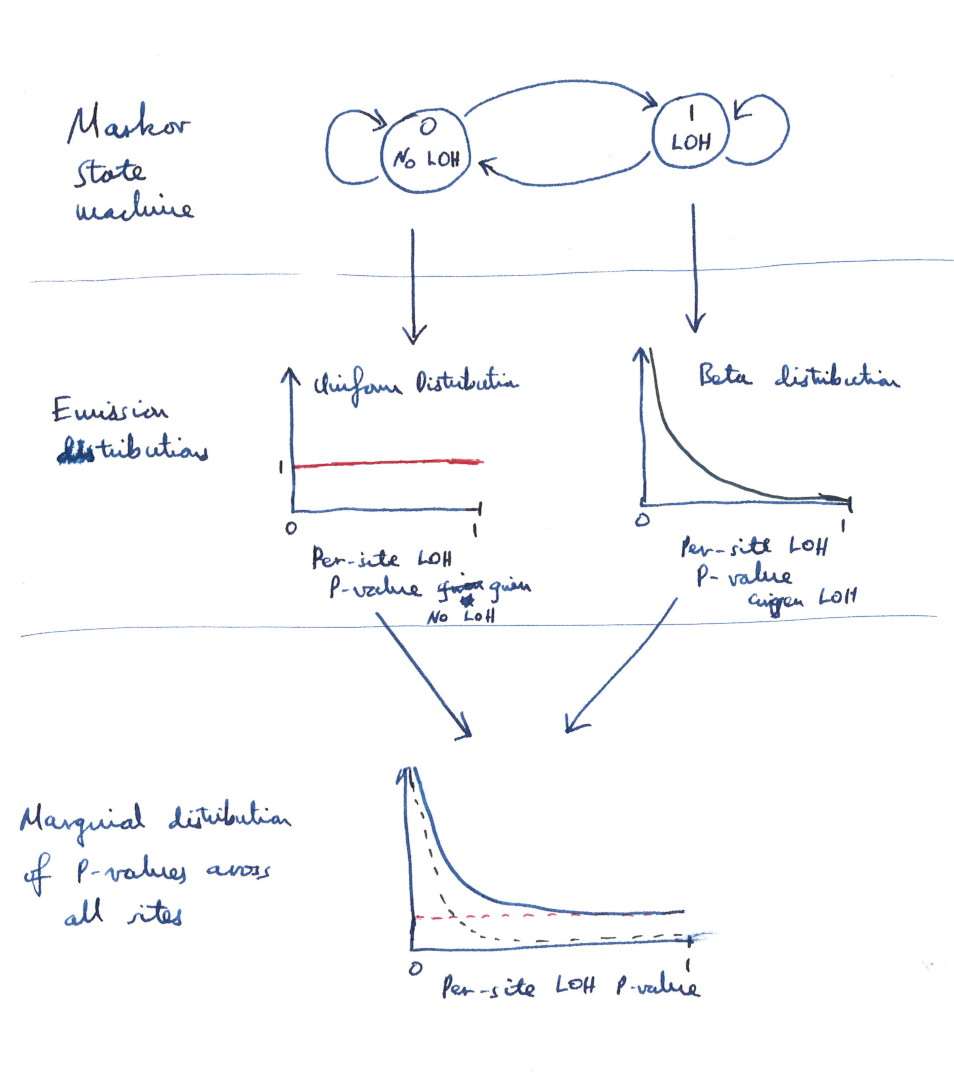
\includegraphics[width=100mm]{resources/comp_loh_hmm.jpg}
\caption{Locality-sensitive FDR estimation of LOH calls using a Markov chain Beta-Uniform mixture model.\label{fig:comp_loh_hmm}}
\end{figure}

Extension of the procedure to the \gls{CNV} case requires three states: \emph{Diploid}, \emph{Loss}, and \emph{Gain} (figure~\ref{fig:comp_cnv_hmm}).  We take advantage of the $W_5$ statistic's symmetry and fit the \gls{HMM} to the one-sided $p_{loss}$ \gls{CNV} P-values; \gls{CNV} loss is then indicated by P-values near zero, and \gls{CNV} gain by P-values near one.  The \emph{Loss} and \emph{Gain} states are modelled by Beta distributions, left-skewed in the \emph{Loss} case, and right-skewed in the \emph{Gain} case.  The posterior probability of a locus being in state \emph{Diploid} then gives the overall \gls{FDR} for a \gls{CNV} call at that locus.  \Gls{BIC} model selection is performed as for the \gls{LOH} case, except in this case four models are compared: \emph{Diploid}, \emph{Diploid / Loss}, \emph{Diploid / Gain}, and \emph{Loss / Diploid / Gain}.
\begin{figure}[!htbp]
\centering
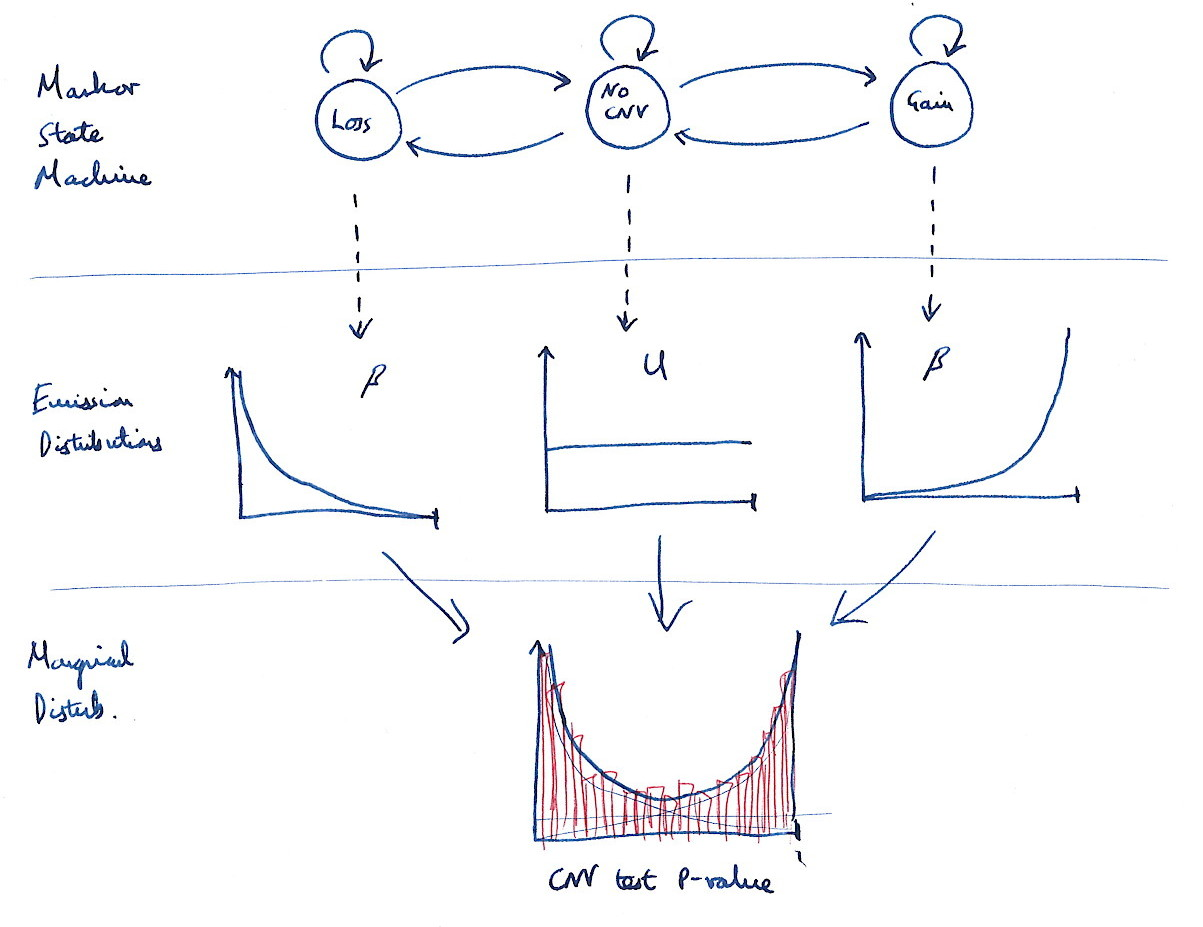
\includegraphics[width=100mm]{resources/comp_cnv_hmm.jpg}
\caption{Locality-sensitive FDR estimation of CNV calls using a Markov chain double-Beta-Uniform mixture model.\label{fig:comp_cnv_hmm}}
\end{figure}

Although the given procedure is simple in formulation, some additional complexities were required for a practical implementation, all related to the high degree of flexibility of the Beta distribution.  The Uniform distribution is a special case of the Beta distribution, and therefore in cases where the distribution of P-values is near Uniform (ie. all sites appear to satisfy the null hypothesis), the fitting problem is ill-posed.  This issue was resolved by enforcing Beta parameters $\alpha \leq 0.95$ for \gls{LOH} and \gls{CNV} loss detection, and $\beta \leq 0.95$ for \gls{CNV} gain detection.  For \gls{FDR} correction of \gls{CNV} P-values, structural zeros were placed on the probabilities of direct transitions between \emph{Loss} and \emph{Gain} states (figure \ref{fig:comp_cnv_hmm}); although such transitions are biologically plausible, they were found to contribute to unstable fits in noisy data.

%\bibliographystyle{plain}
%\bibliography{thesis}

\end{document}
